\documentclass[letterpaper,12pt]{article}
\usepackage[margin=0.75in]{geometry}
\usepackage{amssymb}
\usepackage{amsmath}
\usepackage{setspace}
\usepackage{titlesec}
\usepackage{lipsum}
\usepackage{float}
\usepackage{physics}
\usepackage{subfig}
\usepackage{graphicx}
\usepackage{multicol}
\usepackage[table,xcdraw]{xcolor}

\title{Social Robot}
\author{\textbf{Professor:} \\  Dr. Ashraf Gaffar \\
\\
  \textbf{Working Group: (Team \#4)} \\
  Aishwarya Pratap Singh (1211162781) \quad Pradeep Kumar (1211519631) \\
  Vidhi Patel (1209261712) \quad Nikhil Lohia (1211168085) \\
  Naveen Piedy (1210844645) \quad Akil Kumar (1211165030) \\
  Saranya Damodaran (1211093179) \quad Jiuxu Chen (1211669885)}

\date{December 3, 2016}
\providecommand{\keywords}[1]{\textbf{\textit{Keywords---}} #1}
\begin{document}

\thispagestyle{empty}
\maketitle

\begin{multicols}{2}

\section{Abstract}
\textit{Artificial intelligence has contributed to a gamut of applications in today's world. This has already started to affect our daily life in ways that we could not even have begun to contemplate only a hundred years ago. Whilst there are many advances in this field of study which has a major impact on the society. These AI improvements will enable ubiquitous robotics which is major transition to robot-like companions. Social robot interacts and communicates with humans and other agents based on the instructions given to it. In the following sections we talk about the features of the social robot and the benefits towards the contributions.}

\section{Introduction}
Artificial intelligence has created fascinating models of social robot that can be possibly used for interaction with the environment and other agents. The robot can interact in a social manner even though there is no explicit communication. The advancement in artificial intelligence has taken a step to understand the underlying mechanisms involved in thought and intelligence and their embodiment in machines. These advancements will allow the agents to reason and interact with the world. The applications are widespread across various disciplines such as engineering, natural sciences, economics, business, e-learning, healthcare etc. Artificial intelligence covered a large extent of applications in the field of software engineering. It has brought a significant development in all the phases of the software development life cycle including the methodologies, programming languages and environment has made a significant progress. \\
\par
Social robot is the physical model of human facial muscles that responds to input and display emotions based on the input provided to it. A physical robot is developed using technology like 3D printers which enables smaller batches of highly customized components. These components are buildable into a whole robot which is programmed using sensors, motors and controllers. 

\section{Getting Started}
Social robot has been built by assembling various components that was 3D printed. These 3D printed components are assembled to build the whole robot that can move and actually do things. The various components that were printed to build the robot include a head base, neck base, neck joint, eye mechanism, eyelids, eyeball, upper jaw and lower jaw. The temperature of the machine has to be set appropriately for the kind of plastic that is used for printing the 3D components. The components are assembled along with the servo motors. Servo motors are rotary actuator that allows for precise control of angular or linear position, velocity and acceleration. These servo motors are controlled by sending an electrical pulse through control wire. A servo motor can usually rotate 180 degrees when it receives the electrical pulse. There are two types of servos that are used in building the social robot. One of them is a little servo motor that is used for eyes, eyebrows and mouth. The second one is a $1501MG$ servo motor that are bigger, higher-torque servos that are used to move the whole head. These servo motors are controlled by the wires which are connected to the microcontroller. The microcontroller is programmed to control the robot. In order to program the microcontroller, PSOC creator is used to write embedded C programs. These are then fed into the microcontroller to control the robot

\section{3D Printing}
3D printing is considered as an additive process. Additive process is a way of laying down successive layers of material until the object is created. These layers are hence thinly sliced horizontal cross-section of the object. In order to start with 3D printing, a virtual design of the object is required. These virtual designs are then fed into the 3D printing once the plastic is loaded into the printer. The time taken to print these objects vary depending on the size of the object that is required to print. The kind of 3D printer, that is used here to print the components, uses a methodology of melting or softening the material to produce the layers. The object that has to be printed is done by extruding the melted material. The melted material forms layers that hardens immediately. The material extrudes from a nozzle in the machine. With this magnum of application, 3D printing will allow an idea to develop faster which would have taken months otherwise. This also helps to verify a design before investing in a model. That is a prototype can be created redesigned and alter an existing mold.

\section{Components}
These components are then fixed in the appropriate sockets to build the whole robot. Along with these components, the mechanical and electrical components are also attached. The brass rods are cut to length to connect servo horns to the ball joints in the eye mechanism. Along with this a bushing is used as a linear bearing which is connected to a 8 mm rod that supports back and forth movement to replicate blinking. In order to allow rotation in the eyeball, the ball connectors are attached to the printed ball sockets. Primarily, universal joint is used to connect the head to the neck. Other than the mechanical components, the electrical components that has been used are servo motors that are used for eyes, eyebrows, mouth and higher-torque servos to move the whole head. To make these servos work, a 5V power supply is used. Additionally the power is supplied to the controller that is used for the robot. These servo motors connected to the microcontroller using a bunch of wires of various colors. These wires are connected to solderless breadboard. This is the microcontroller that will be programmed to control the robot. Further, for the components to be joined into a whole robot acrylic glue is used here and there to hold the parts together. These components are fixed in such way that there is smooth movement in the gestures that the robot is programmed to do. Since, only the skeletal view of the robot is represented, the wires that are connected to each servo motors are always on display.

\section{Structure}
The components that are printed using the 3D printer consists of additional layers called the supporting material. These supporting material hold the mold together while printing the component. Once the mold gets hardened, these supporting materials are then scraped off to enable the components to fix appropriately in the sockets. The lower most component is the lower neck base which forms the base and is attached to the cardboard. Once, the lower neck base has been attached to the cardboard base the upper neck base can be fixed. Along the side of the upper neck base, two servo motors are fixed. These high torque motors enable the neck movement. These two components are fixed together using screws. Now, the upper neck base provides a provision to hold the neck U-joint bracket which serves as the holder for universal joint. Hence, the u-joint bracket is inserted into the socket provided by the upper neck base. \\
\par
The universal joint can finally be fixed in the neck U-joint bracket. Universal joint is a joint or  coupling in a rigid rod that allows the rod to ‘bend’ in any direction and is used in shafts that enables rotary motion. Therefore, the universal joint will allow the head of the robot to rotate in freely. The universal joint in turn holds the head base which serves as a bridge between the neck of the robot and head of the robot. Additionally, the head base has been connected along with threaded rod. These threaded rods are tendons in the neck. In turn, these tendons like threaded rod are screwed to the large servo arm. The high torque servo motors, that are connected to the lower neck base, are connected to the large servo arm. The head base holds a lot of other components like upper jaw, lower jaw and supports for head. The upper jaw is fixed to the upper part of the head base. The upper jaw has two servo motors attached to it which enables the jaw to move up and down. To give a feel of the jaw, a high-temperature silicon rubber tube is attached on the face of the jaw. Likewise, the lower jaw is fixed to the servo motor and a high-temperature silicon rubber tube attached around it. Now, to hold eye-mechanism a component called head support is attached to the head base as well. There are two head supports called the head support left and head support right. These two head supports are attached on either side of the head base. \\
\par
Once, all these components are in place the eye mechanism is fixed on the other end of the head support. The eye mechanism holds a lot of other components which forms the major part of the robot. To start with, the eye mechanism consists of the eyes and eyebrows. Eyes are constructed using eyelids and eyeballs which were printed using the 3D printer. These components initially consists of the supporting materials which are scraped off before assembling them together. To hold the eye socket, the eyeball U-joint is fixed to the eye mechanism. Once the eyeball U-joint is fixed, the eyeball is fixed to the U-joint. This is fixed by screwing the eyeball socket to the eyeball U-joint extended square that is found inside the eyeball. The eyelid set are then fixed on the eyeball in such a way it replicates the eyes. These eyelids are connected to the servo motors to make the eyelids move up and down to replicate the closing and opening of the eyes. These movements are facilitated by rods that moves to and forth to move the eyelids up and down. The servo motor are connected to these rods which allows the rods to move smoothly. This movement is controlled by one servo motor. Whereas, the eyeball movements are controlled by two servo motors with the help of rods that are connected to the eyeball. \\
\par
Additionally, the blink mechanism bearing will facilitate the blink movements of the robot. Moreover, the expressions of the robot are further bolstered with the use of eyebrows. The eyebrow component is fixed to the eye mechanism to hold the servo motors that controls the movement of the eyebrow. For the eyebrow, a high-temperature silicon rubber tube is used and is connected to the servo motors. There are two servo motors that are used for each eyebrow to control the eyebrow movement. Various emotions can be expressed with various positions of the eyebrows. \\
\par
Thus a social robot that replicates the human emotions are developed using a set of servo motors, wires, components and programmable microcontroller. \\

\begin{figure}[H]
\begin{center}
\subfloat[Diagram]{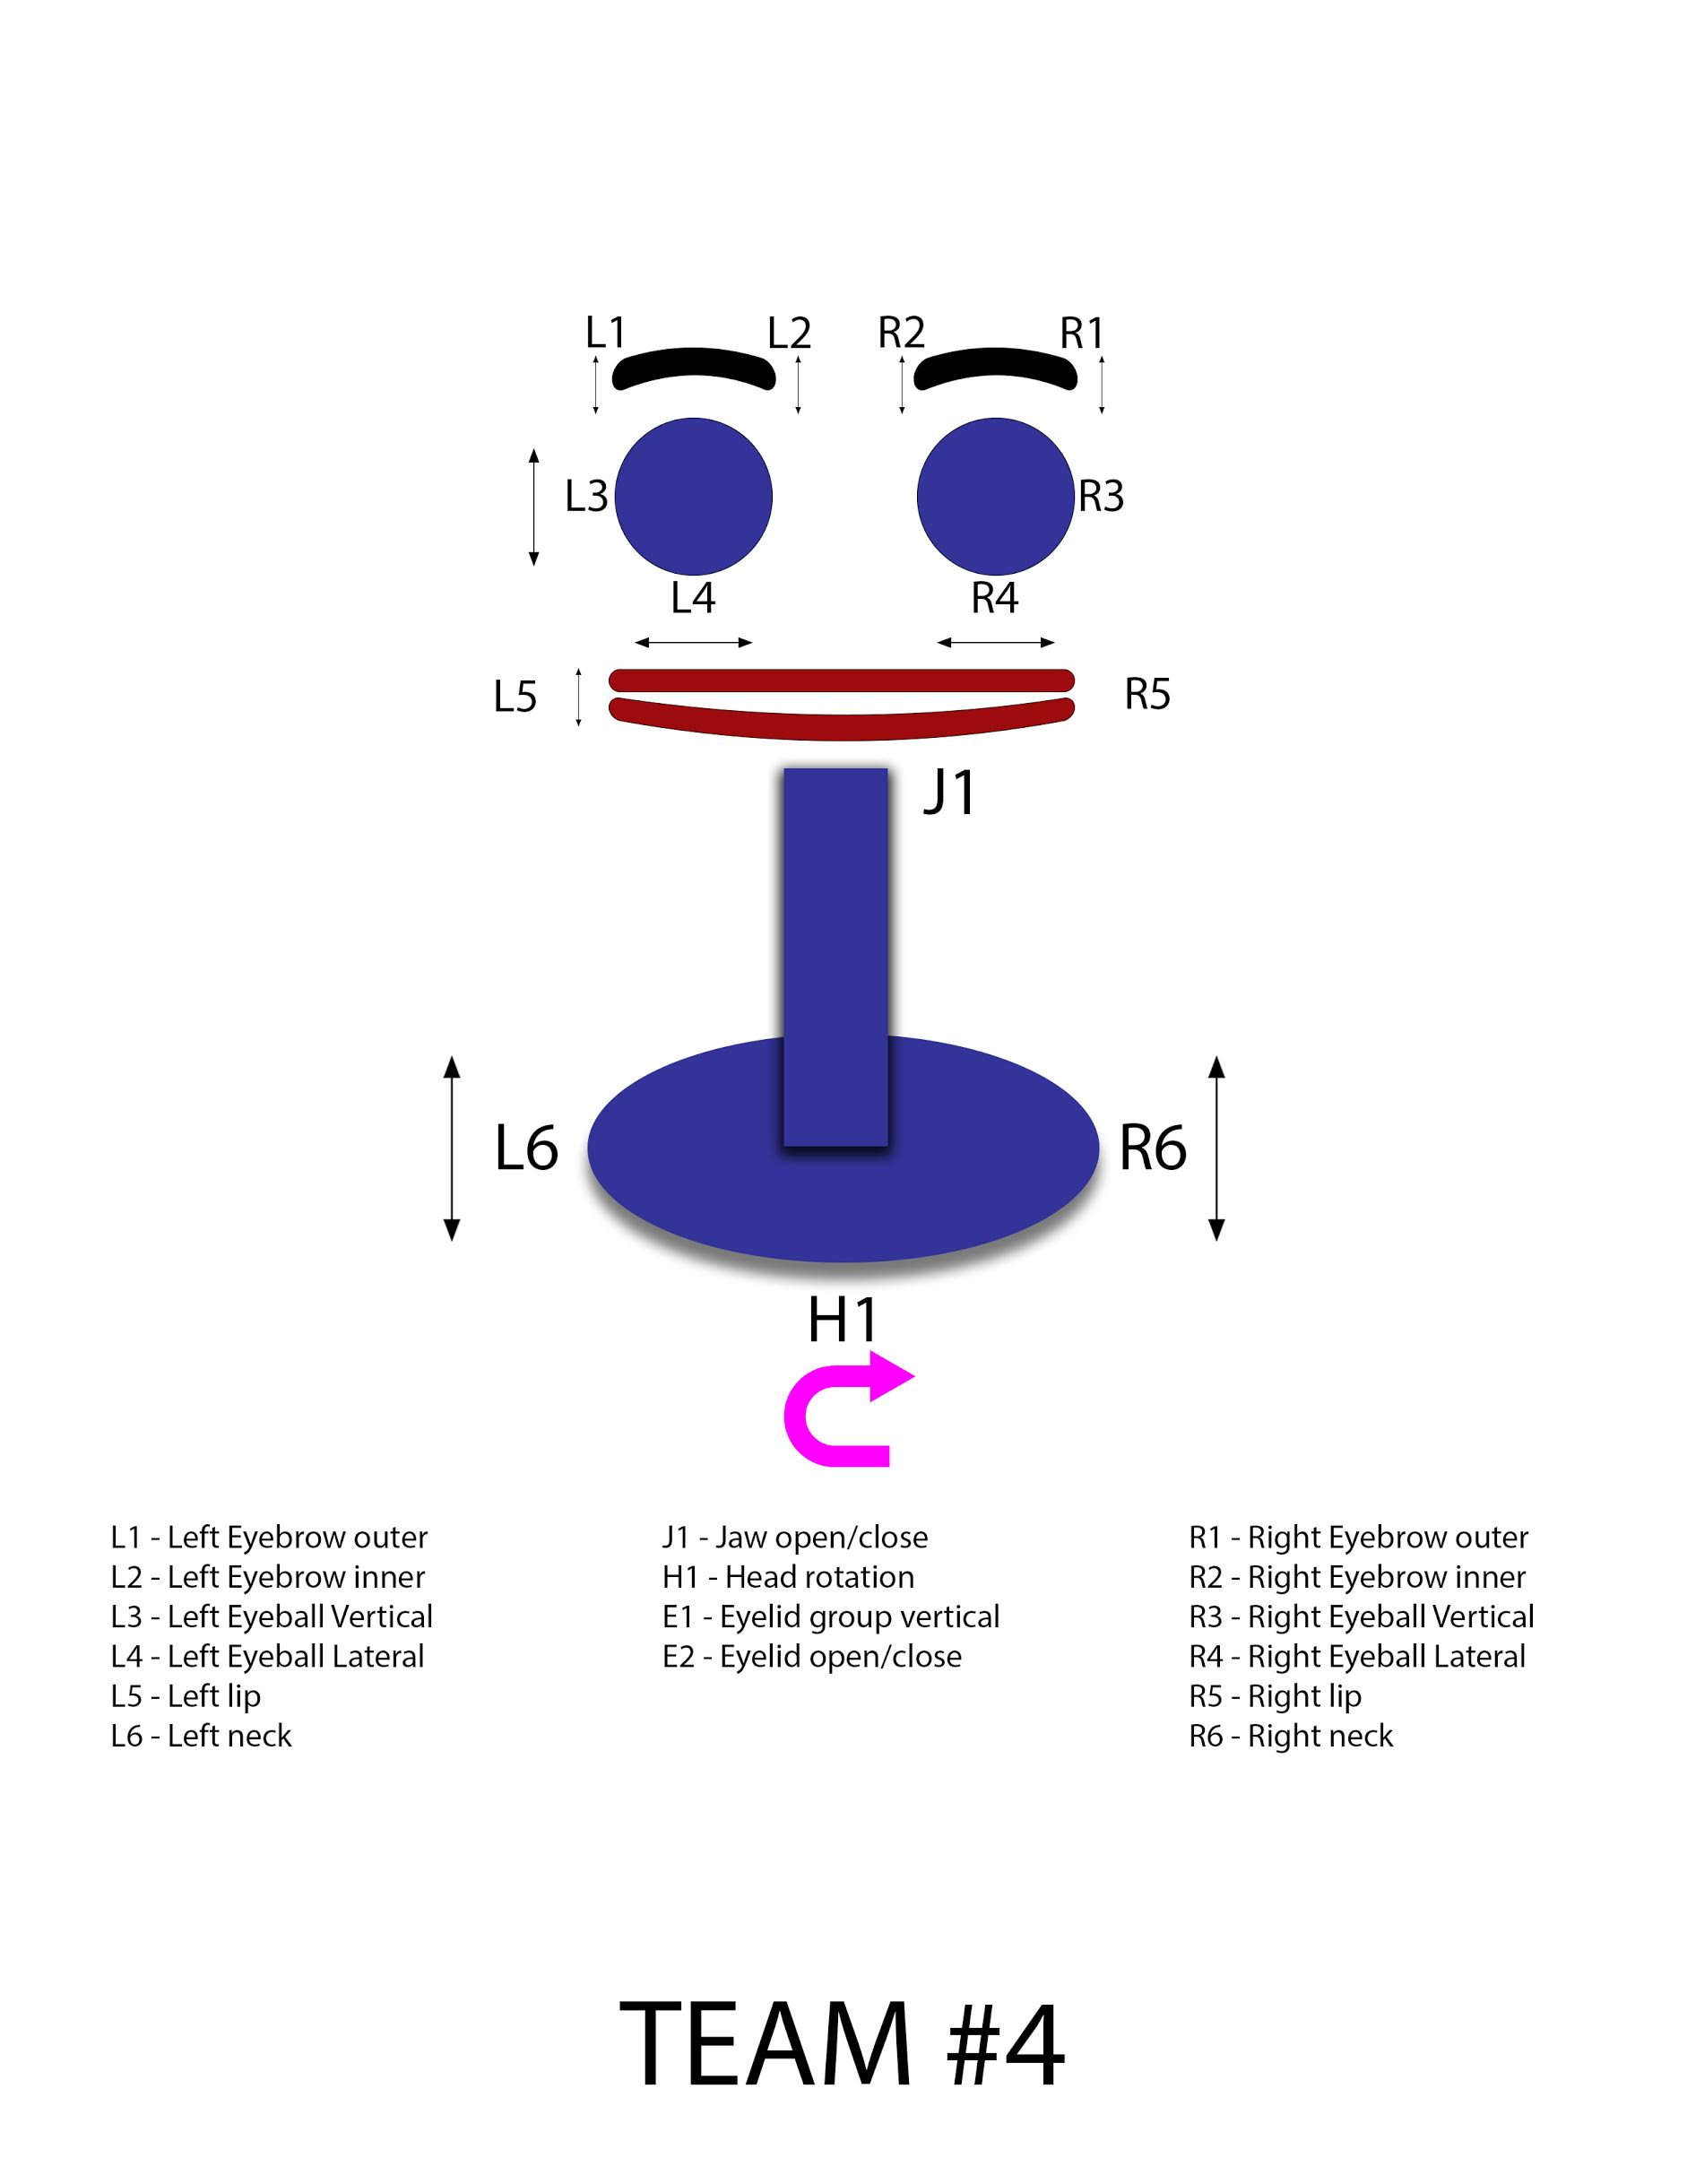
\includegraphics[width = 2in]{robot_blue}}
\end{center}
\caption{Blueprint of the robot}
\end{figure}

\begin{figure}[H]
\begin{center}
\subfloat[Diagram]{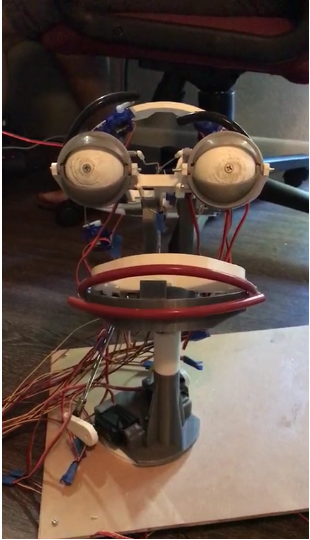
\includegraphics[width = 1.25in]{robot}}
\end{center}
\caption{Completed robot}
\end{figure}


\section{Programming}
Programmable microcontroller is used to control the servo motors by sending them pulse width modulation(PWM). PWM is a modulation technique that is used to encode a message into pulsing signal. Therefore, these signals are used to supply power to electrical devices such as motors. According to wikipedia, pulse-width modulation uses a rectangular pulse wave whose pulse width is modulated resulting in the variation of the average value of the waveform. The average value of the waveform is given by:
\begin{equation}
y = \frac{1}{T}\int_{0}^{T}f(t) dt
\end{equation}
As $f(t)$ is a pulse wave, its value is $y_{max}$ for $0 < t < D.T$ and $t_{min}$ for $D.T < t < T.$ The above expression then becomes
\begin{equation}
y = \frac{1}{T}\left(\int_{0}^{DT}y_{max}dt + \int_{DT}^{T}y_{min}dt\right)
\end{equation}

\begin{equation}
= \frac{1}{T}\left(D.T.y_{max} + T(1-D)y_{min}\right)
\end{equation}

\begin{equation}
= D.y_{max} + (1-D).y_{min}
\end{equation}
PWM is used to control the servo motors which is a three-wire connection where two wires are for DC supply and the other one for carrying the pulses. These pulses are sent from PSoC which is a embedded system-on-chip integrating an MCU core. A PSoC integrated circuit consists of core, configurable analog and digital blocks, and programmable routing and interconnect.\\
\par
PSoC creator is an IDE that is used to design debug and program the devices. PSoC creator allows user to select, configure and connect existing circuits on the chip and components. This allows users with great ease to design and learn the working of the microcontroller. For programming the microcontroller, a PSoC creator 4.0 is used. At the start of the project, PSoC 5 LP is chosen since we are programming a robot controller. We are required to send across signals to the servo motors with pulse width modulation. Therefore we choose PWM functions to drag and drop the objects on the grid design space. PMW uses 5 interfaces such as two left interfaces which includes clock and reset. The other three interfaces are TC, PWM1 and PWM2. These interfaces are used to connect to the components. For instance, the clock can be wired to the clock interface. To do so the clock is dragged and it is aligned with the clock interface and make sure they are both visually connected. To wire the reset interface, connect the logic low to PWM reset interface. Next is to connect the output pins to PWM1 and PWM2 interfaces. In order to do so, the digital output pin is dragged and connected to PWM1 and PWM2 interfaces of the PWM object. Various PWM objects are created for the robot and they are left eyebrow, right eyebrow, left eyeball, right eyeball, lip, jaw, neck and head. Each of these objects consists of tc, clock, reset and interrupt. The clock input defines the signal to count. This counter is increased or decreased on each rising edge of the clock. The reset input is a period counter and it continues normal operation. Whereas, tc is the output which is the terminal count output. The terminal count output is `1' when the period counter is equal to zero. If the PWM is stopped with the period counter equal to zero then this signal will remain high until the period counter is no longer zero. The interrupt output is the logical OR of the group of possible interrupt sources. PWM/PWM1 output is the first or only pulse width modulated output. This signal is defined by PWM mode, compare modes as indicated in the waveforms. PWM2 output is the second pulse width modulated output. This output is only visible when the PWM mode is set to ``Two Outputs''.\\
\par
Few configurations has to be made before the microcontroller can be programmed. The compare values are defined as 0. These values define the compare output functionality in conjunction with the hardware Compare Type options. The compare values may be changed at any time by the PWM\_WriteCompare1(comparevalue) and PWM\_WriteCompare2(comparevalue) API calls. These parameters hold only the initial value written during configuration. The CMP1 and CMP2 are compare value parameters which define the two period counter comparisons that make up the PWM outputs. \\
\par
Variations are made when a pulse is sent to a servo that controls the movement of the servo between 0 to 180 degrees. These pulses ranges from 0.65ms to 2.60ms which controls 0 to 180 degree movement respectively. It rotated the servo to a position and holds its output shaft some number of degrees counterclockwise from the neutral point. Further, the CWDR tab displays port list which is numbered from P0 to P15. Once, all the ports are connected to corresponding motors, the microcontroller is programmed by specifying the WriteCompare APIs. Once, the compare values have been coded, the code should build and run smoothly. \\
\par
Once the code has been successfully built, the wires are connected to the servo motors. These servo motors will respond by showcasing various movements. These movements are combined motions of eyebrows, eyelids, mouth and neck.



\section{CONCLUSION}
Social and interactive skills are necessary in many application areas where robots need to interact and collaborate with humans and other agents. For instance, interactive robots can be used in e-learning environment. As new technologies are evolving, there are demands to ease the day-to-day activities which otherwise will slow down the fast moving world. Eventually, the demand for incorporating artificial intelligence into machines that can be used to substitute the human activities. Artificial intelligence can be incorporated in E-learning which will be individualized for each student allowing for better differentiation and allowing students to work for mastery at their own pace. As technologies advance, the robots are designed to be adaptive where it can change and respond to a fluctuating environment. These robots can make decisions on its own and continue with its process. Therefore, advancements in this field of study can be designed to a whole lot of things, ranging from delicate and precision tasks. Robots are considered to be super-machines.

\end{multicols}

\begin{thebibliography}{9}
\footnotesize
\setlength{\itemsep}{0pt}
\bibitem{latexcompanion}
M.~Goossens, F.~Mittelbach, A.~Samarin. \emph{The \LaTeX\ Companion},
Addison-Wesley (1994), ISBN~0-201-54199-8.

\bibitem{}
http://www.cypress.com/products/microcontroller-mcu-and-programmable-system-chip-psoc-families
\bibitem{}
https://en.wikipedia.org/wiki/Pulse-width\_modulation
\bibitem{}
http://www.cypress.com/file/131701/download
\bibitem{}
https://pdfs.semanticscholar.org/4636/0023613e1c12f993065739dbd54192a1fcff.pdf
\bibitem{}
http://www.brighthubengineering.com/robotics/26215-robotics-scope-and-limitations-of-robots/

\end{thebibliography}

\end{document}
